\documentclass{source/Report}
\usepackage{caption}
\usepackage{multirow}

\major{信息工程}
\name{张卓雨}
\title{}
\stuid{3210105816}
\college{信息与电子工程学院}
\date{2023年3月30日}
\lab{东四-420}
\course{电磁场与电磁波}
\instructor{吴锡东、王子立}
\grades{}
\expname{矩形波导馈电的角锥喇叭天线CST仿真}
\exptype{仿真实验}
\partner{无}

\begin{document}
\makecover
\makeheader
\section{实验目的}
\begin{enumerate}[label={\arabic*.}]
    \item 了解并掌握波导喇叭天线的常用分析指标和分析方法。
    \item 熟悉CST软件的基本使用方法,并能够应用其对特定的微波器件或电路进行建模、仿真分析。
\end{enumerate}

\section{实验原理}
\subsection{喇叭天线概述}
喇叭天线是一种应用广泛的微波天线,其优点是结构简单、频带宽、功率容量大、调整与使用方便。合理的选择喇叭尺寸,可以取得良好的辐射特性:相当尖锐的主瓣,较小副瓣和较高的增益。因此喇叭天线在军事和民用上应用都非常广泛,是一种常见的测试用天线。喇叭天线的基本形式是把矩形波导和圆波导的开口面逐渐扩展而形成的,由于是波导开口面的逐渐扩大,改善了波导与自由空间的匹配,使得波导中的反射系数小,即波导中传输的绝大部分能量由喇叭辐射出去,反射的能量很小。
\subsection{矩形波导馈电角锥喇叭天线}
角锥喇叭天线是对馈电的矩形波导在宽边和窄边均按一定的角度张开形成的天线,其结构示意图如图1所示。矩形波导的尺寸为 $a\times b$ ,喇叭口径尺寸为 $D_H\times D_E$ ,喇叭高度为 $L$ 。
\begin{figure}[H]
    \begin{center}
        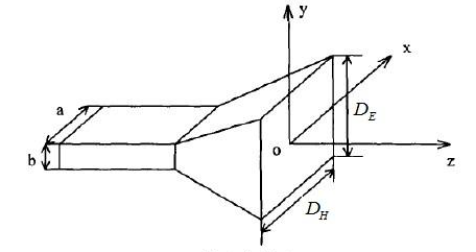
\includegraphics[width=0.4\linewidth]{pic/cb2_p1.png}
        \caption{}
    \end{center}
\end{figure}
对于矩形波导尺寸为 $a\times b$ ,喇叭口径尺寸为 $D_H\times D_E$ ,喇叭高度为 $L$ 的角锥喇叭天线,可以用以下公式来估算喇叭的增益:
$$G=0.51\dfrac{4\pi A_p}{\lambda^2}$$
其中 $A_p$ 为喇叭的物理口径 $D_H\times D_E$ 。
\section{实验设备}
装有CST软件的电脑\qquad 一台
\section{实验内容}
根据给定的矩形波导喇叭天线尺寸,用 CST 建模,仿真其辐射特性,并与喇叭天线辐射特性测量实验对比分析。
\section{实验步骤及数据记录}
\subsection{建立模型}
(1) 参数设置
\begin{figure}[H]
    \begin{center}
        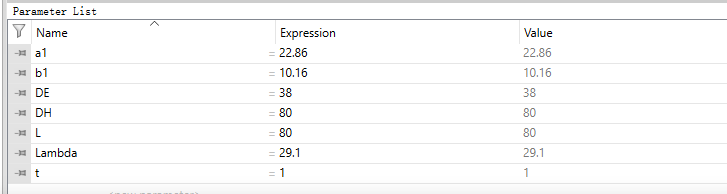
\includegraphics[width=\linewidth]{pic/cb2_p2.png}
        \caption{}
    \end{center}
\end{figure}
(2) 创建矩形
\begin{figure}[H]
    \begin{center}
        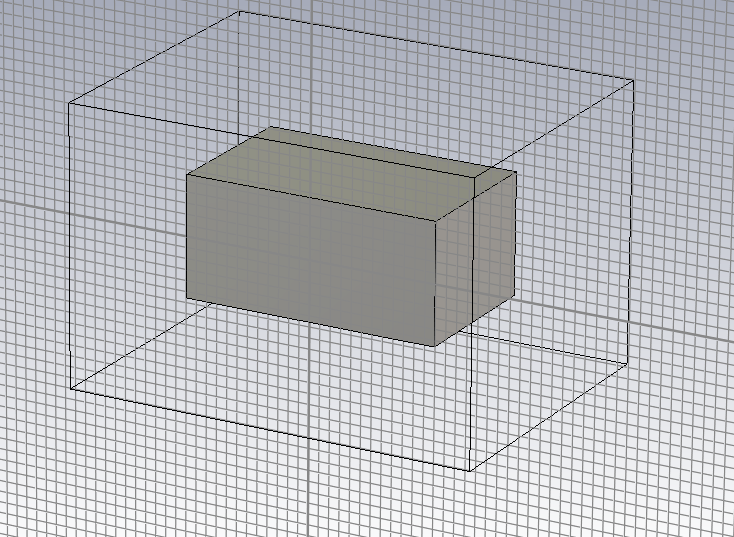
\includegraphics[width=0.45\linewidth]{pic/cb2_p3.png}
        \caption{}
    \end{center}
\end{figure}
(3) 建立喇叭模型
\begin{figure}[H]
    \begin{center}
        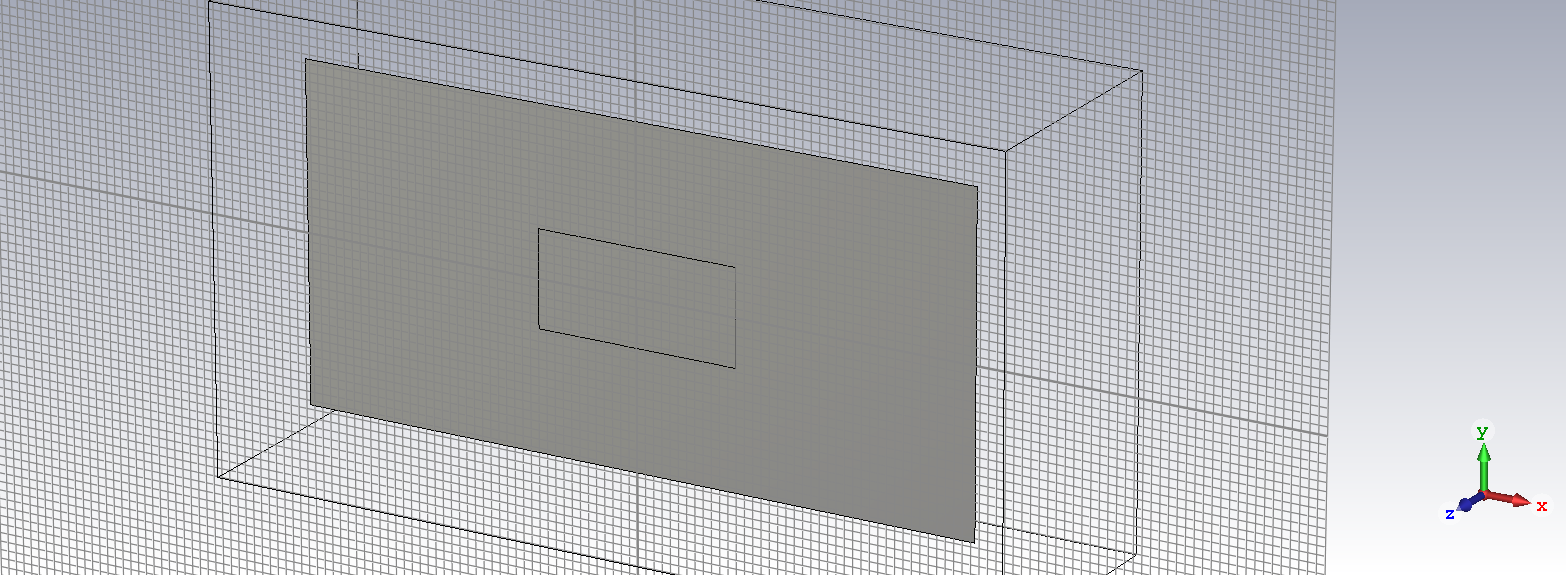
\includegraphics[width=0.7\linewidth]{pic/cb2_p4.png}
        \caption{}
    \end{center}
\end{figure}
(4) 平移
\begin{figure}[H]
    \begin{center}
        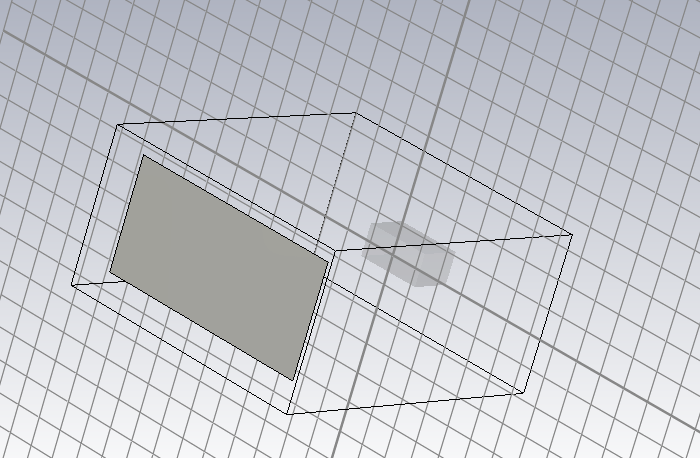
\includegraphics[width=0.45\linewidth]{pic/cb2_p5.png}
        \caption{}
    \end{center}
\end{figure}
(5) 生成喇叭形状
\begin{figure}[H]
    \begin{center}
        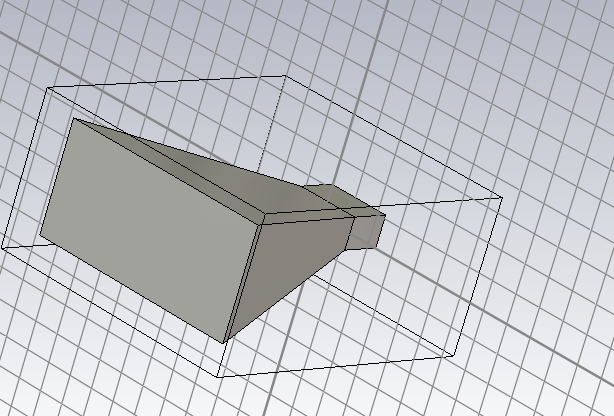
\includegraphics[width=0.45\linewidth]{pic/cb2_p6.png}
        \caption{}
    \end{center}
\end{figure}
(6) 掏空
\begin{figure}[H]
    \begin{center}
        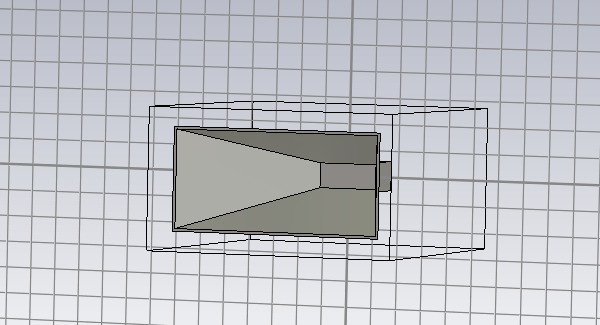
\includegraphics[width=0.45\linewidth]{pic/cb2_p7.png}
        \caption{}
    \end{center}
\end{figure}
\subsection{仿真}
(1) 仿真设置\par
仿真频率设置:
\begin{figure}[H]
    \begin{center}
        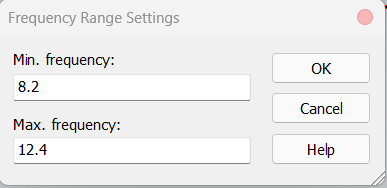
\includegraphics[width=0.35\linewidth]{pic/cb2_p8.png}
        \caption{}
    \end{center}
\end{figure}
仿真背景设置:
\begin{figure}[H]
    \begin{center}
        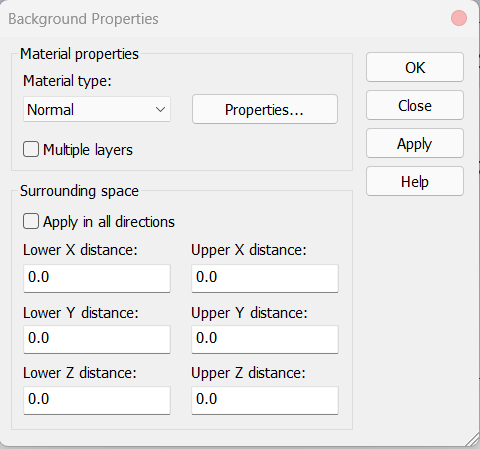
\includegraphics[width=0.4\linewidth]{pic/cb2_p9.png}
        \caption{}
    \end{center}
\end{figure}
仿真边界条件设置:
\begin{figure}[H]
    \begin{center}
        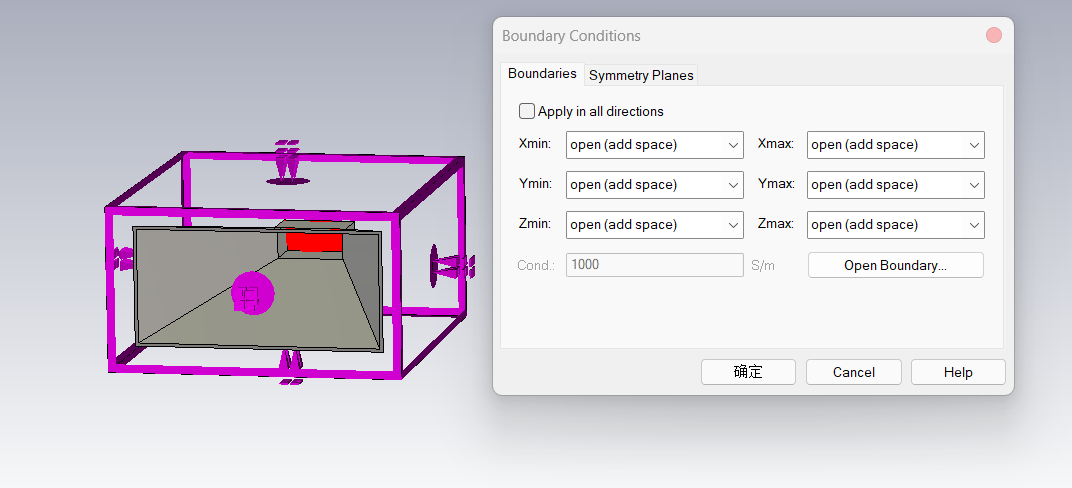
\includegraphics[width=0.8\linewidth]{pic/cb2_p10.png}
        \caption{}
    \end{center}
\end{figure}
端口及监视器设置:
\begin{figure}[H]
    \begin{center}
        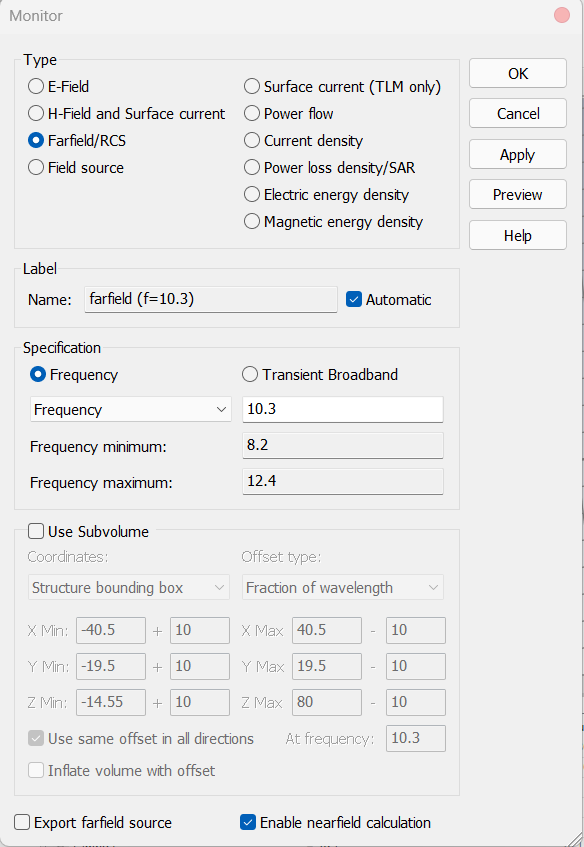
\includegraphics[width=0.45\linewidth]{pic/cb2_p11.png}
        \caption{}
    \end{center}
\end{figure}
求解器设置:
\begin{figure}[H]
    \begin{center}
        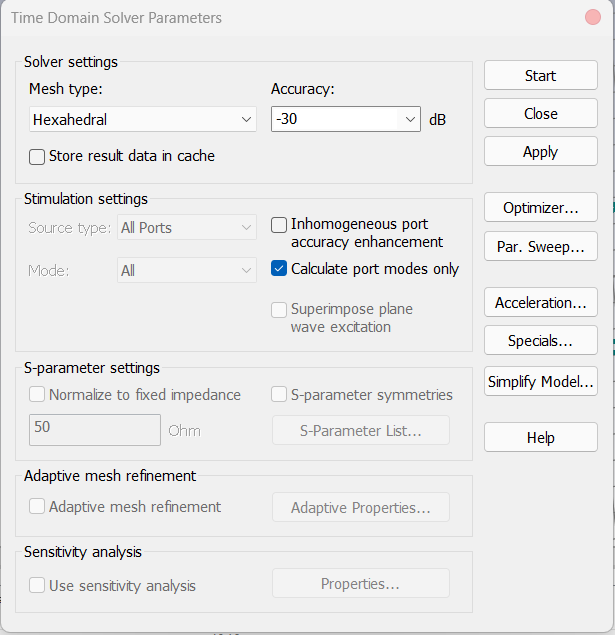
\includegraphics[width=0.8\linewidth]{pic/cb2_p12.png}
        \caption{}
    \end{center}
\end{figure}
\section{实验结果及分析}
\subsection{模式仿真分析}
\begin{figure}[H]
    \begin{center}
        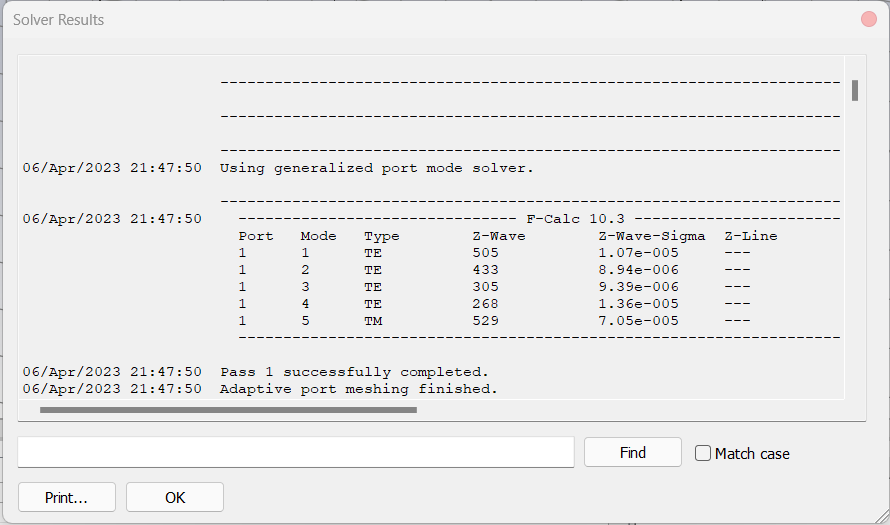
\includegraphics[width=0.8\linewidth]{pic/cb2_p13.png}
        \caption{}
    \end{center}
\end{figure}
由结果知模式数大于1,因此合理。
\subsection{喇叭天线方向图分析}
\begin{figure}[H]
    \begin{center}
        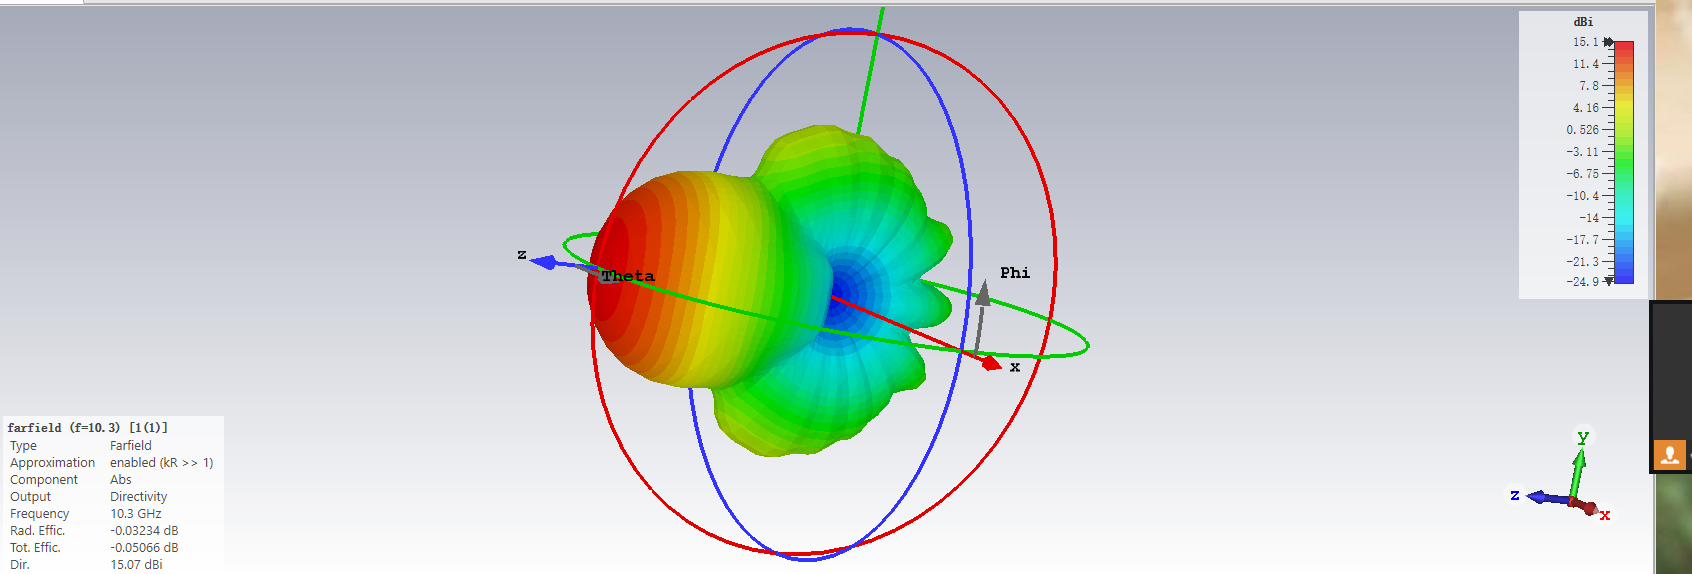
\includegraphics[width=0.8\linewidth]{pic/cb2_p14.png}
        \caption{}
    \end{center}
\end{figure}
\begin{figure}[H]
    \begin{center}
        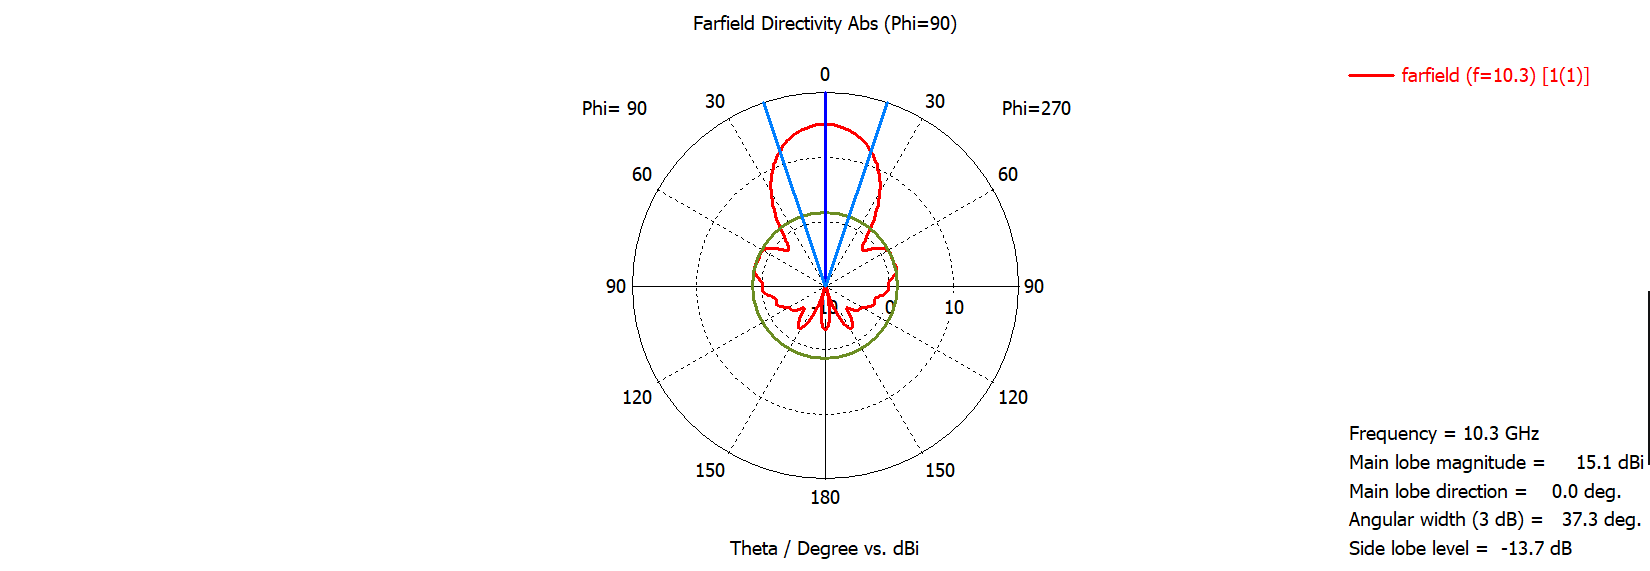
\includegraphics[width=0.6\linewidth]{pic/cb2_p15.png}
        \caption{}
    \end{center}
\end{figure}
由方向图可知,该喇叭天线的主瓣方向为 $\varphi =0^{\circ},\theta =0^{\circ}$ ,主瓣宽度 $37.3^{\circ}$ 。与理论值十分接近。
\subsection{$S_{11}$ 和驻波比特性曲线分析}
\begin{figure}[H]
    \begin{center}
        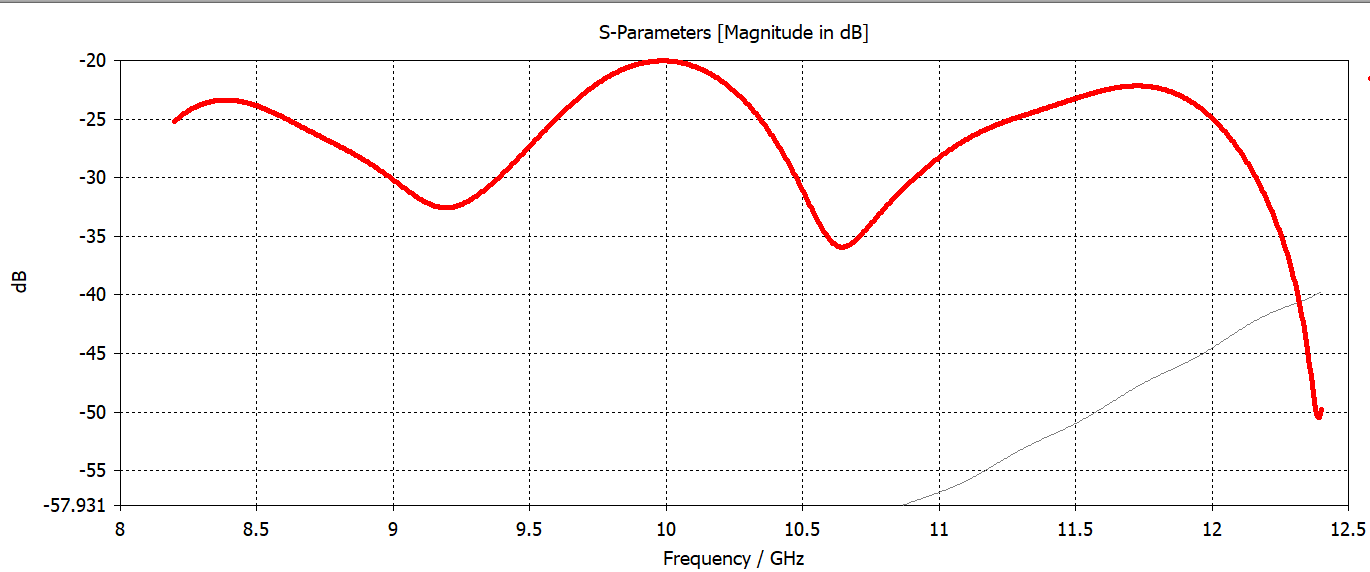
\includegraphics[width=0.8\linewidth]{pic/cb2_p16.png}
        \caption{}
    \end{center}
\end{figure}
\begin{figure}[H]
    \begin{center}
        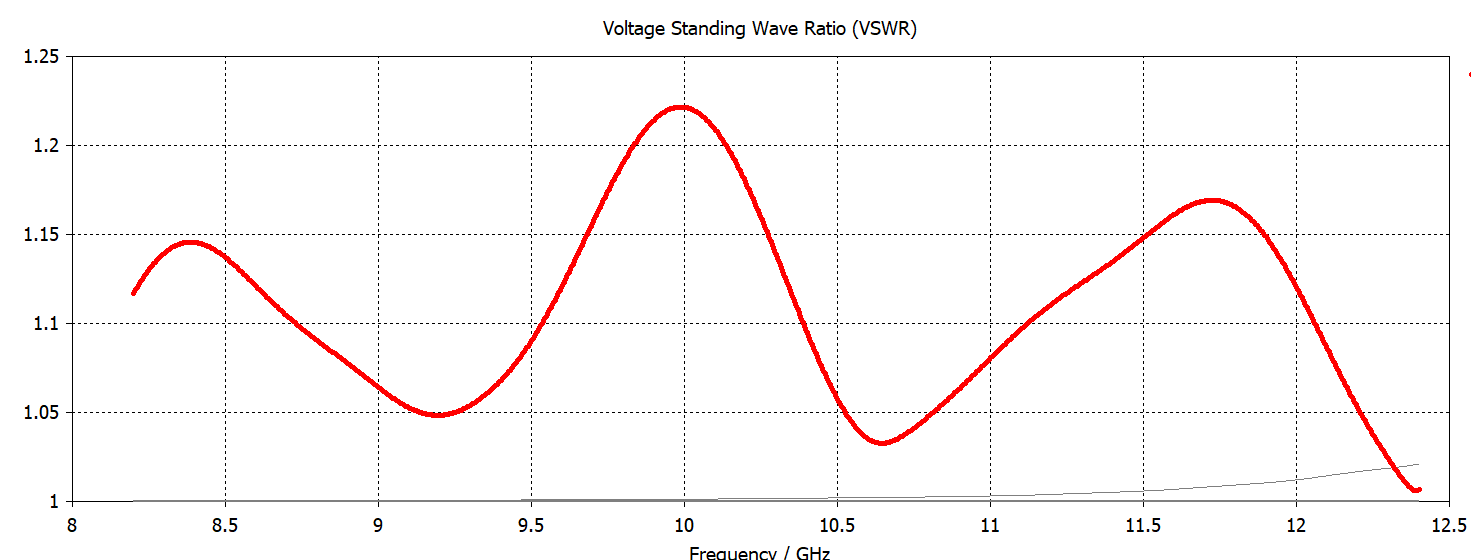
\includegraphics[width=0.8\linewidth]{pic/cb2_p17.png}
        \caption{}
    \end{center}
\end{figure}
\subsection{喇叭天线增益分析}
\begin{figure}[H]
    \begin{center}
        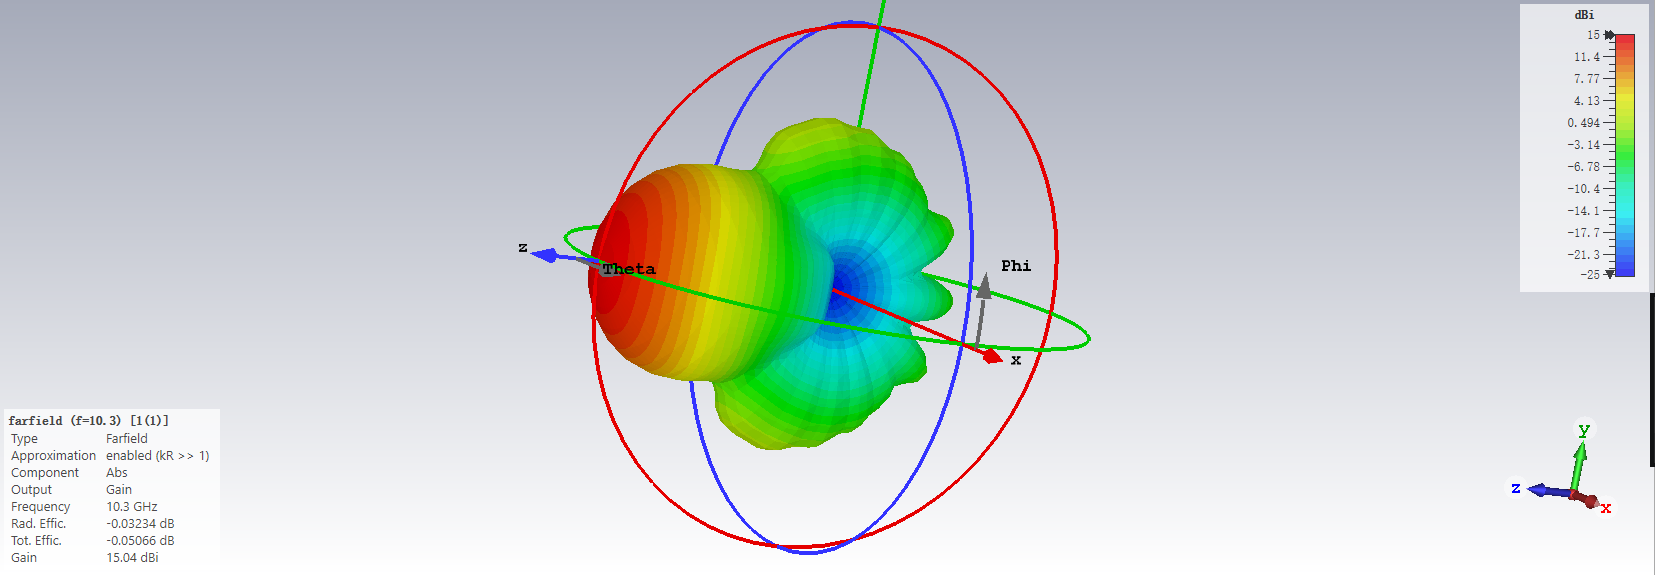
\includegraphics[width=0.8\linewidth]{pic/cb2_p18.png}
        \caption{}
    \end{center}
\end{figure}
\begin{figure}[H]
    \begin{center}
        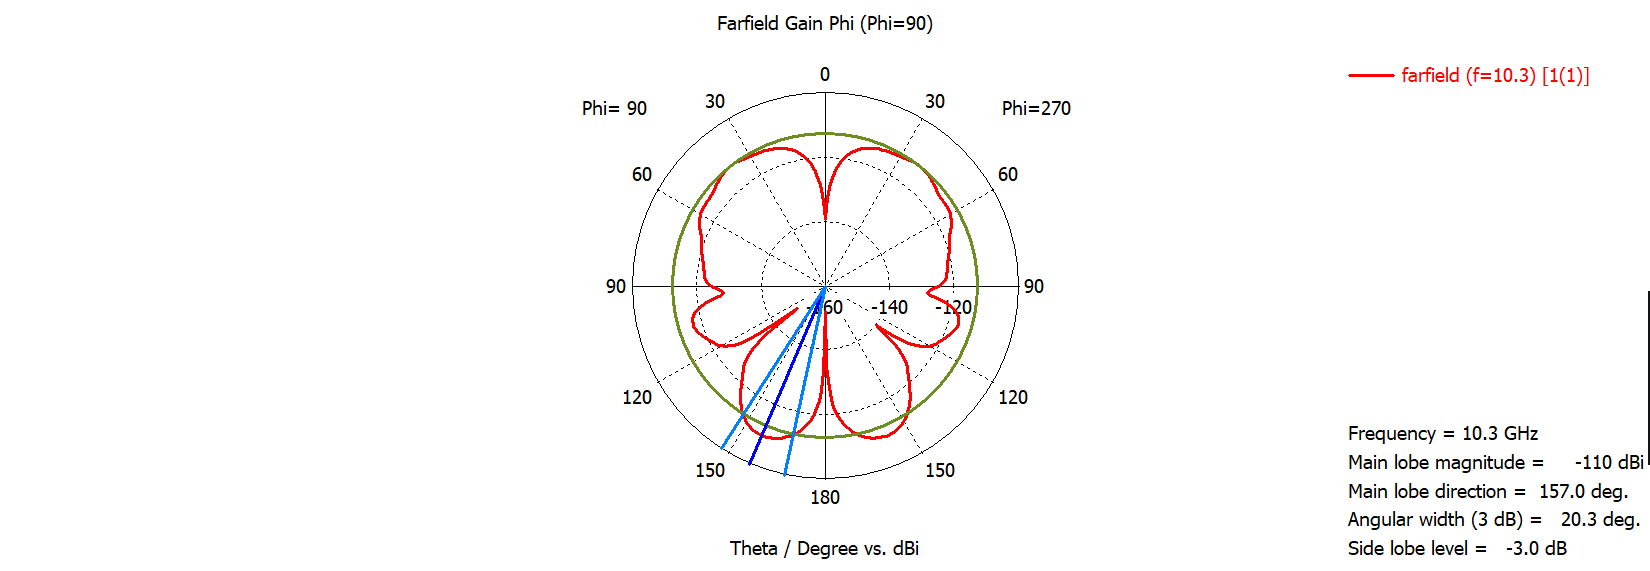
\includegraphics[width=0.8\linewidth]{pic/cb2_p19.png}
        \caption{}
    \end{center}
\end{figure}
仿真结果增益为15.04dB,而理论计算得增益为
$$G=0.51\dfrac{4\pi A_p}{\lambda^2}=23\text{dB}$$
因此二者相差不大,推测误差是由于理论计算模型不够精确造成。
\subsection{喇叭天线和波导口电场情况分析}
\begin{figure}[H]
    \begin{center}
        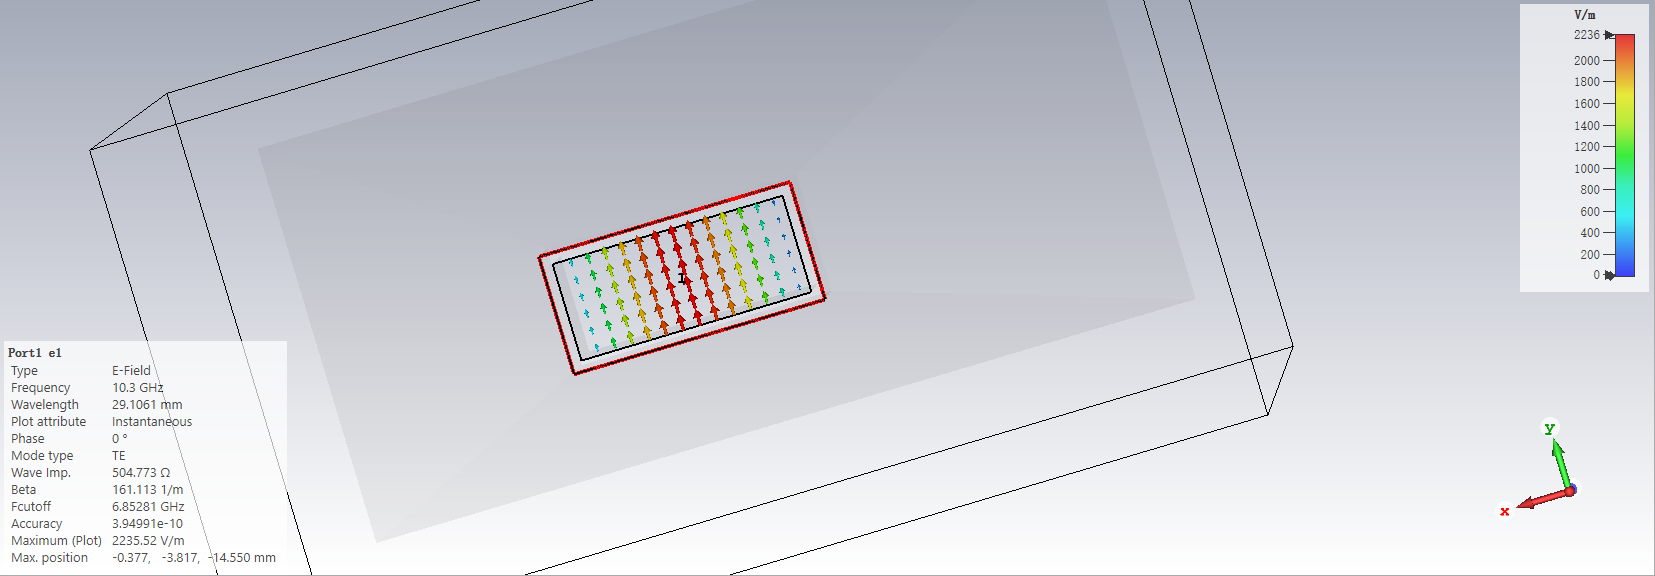
\includegraphics[width=0.8\linewidth]{pic/cb2_p20.png}
        \caption{}
    \end{center}
\end{figure}

\section{实验收获与体会}
在本次实验中,我对CST软件仿真的使用有了一定的理解,但由于理论课还没有学到波导这一章,因此对实验所涉及到的理论一无所知,在做实验时也遇到了许多问题,走了许多弯路,后续应该在学完理论课之后重新做一遍这个实验加深理解。

\end{document}